\documentclass[14pt,a4paper,report]{report}
\usepackage[a4paper, mag=1000, left=2.5cm, right=1cm, top=2cm, bottom=2cm, headsep=0.7cm, footskip=1cm]{geometry}
\usepackage[utf8]{inputenc}
\usepackage[english,russian]{babel}
\usepackage{indentfirst}
\usepackage[dvipsnames]{xcolor}
\usepackage[colorlinks]{hyperref}
\usepackage{listings} 
\usepackage{fancyhdr}
\usepackage{caption}
\usepackage{amsmath}
\usepackage{latexsym}
\usepackage{graphicx}
\usepackage{amsmath}
\usepackage{booktabs}
\usepackage{array}
\hypersetup{
	colorlinks = true,
	linkcolor  = black
}

\usepackage{titlesec}
\titleformat{\chapter}
{\Large\bfseries} % format
{}                % label
{0pt}             % sep
{\huge}           % before-code


\DeclareCaptionFont{white}{\color{white}} 

% Listing description
\usepackage{listings} 
\DeclareCaptionFormat{listing}{\colorbox{gray}{\parbox{\textwidth}{#1#2#3}}}
\captionsetup[lstlisting]{format=listing,labelfont=white,textfont=white}
\lstset{ 
	% Listing settings
	inputencoding = utf8,			
	extendedchars = \true, 
	keepspaces = true, 			  	 % Поддержка кириллицы и пробелов в комментариях
	language = C++,            	 	 % Язык программирования (для подсветки)
	basicstyle = \small\sffamily, 	 % Размер и начертание шрифта для подсветки кода
	numbers = left,               	 % Где поставить нумерацию строк (слева\справа)
	numberstyle = \tiny,          	 % Размер шрифта для номеров строк
	stepnumber = 1,               	 % Размер шага между двумя номерами строк
	numbersep = 5pt,              	 % Как далеко отстоят номера строк от подсвечиваемого кода
	backgroundcolor = \color{white}, % Цвет фона подсветки - используем \usepackage{color}
	showspaces = false,           	 % Показывать или нет пробелы специальными отступами
	showstringspaces = false,    	 % Показывать или нет пробелы в строках
	showtabs = false,           	 % Показывать или нет табуляцию в строках
	frame = single,              	 % Рисовать рамку вокруг кода
	tabsize = 2,                  	 % Размер табуляции по умолчанию равен 2 пробелам
	captionpos = t,             	 % Позиция заголовка вверху [t] или внизу [b] 
	breaklines = true,           	 % Автоматически переносить строки (да\нет)
	breakatwhitespace = false,   	 % Переносить строки только если есть пробел
	escapeinside = {\%*}{*)}      	 % Если нужно добавить комментарии в коде
}

\begin{document}

\def\contentsname{Содержание}

% Titlepage
\begin{titlepage}
	\begin{center}
		\textsc{Санкт-Петербургский Политехнический 
			Университет Петра Великого\\[5mm]
			Кафедра компьютерных систем и программных технологий}
		
		\vfill
		
		\textbf{Отчёт по лабораторной работе №2\\[3mm]
			Курс: «Администрирование компьютерных сетей»\\[3mm]
			Тема: «Тестирование компьютерной сети на основе TCP/IP»\\[35mm]
			}
	\end{center}
	
	\hfill
	\begin{minipage}{.5\textwidth}
		Выполнил студент:\\[2mm] 
		Бояркин Никита Сергеевич\\
		Группа: 13541/3\\[5mm]
		
		Проверил:\\[2mm] 
		Малышев Игорь Алексеевич
	\end{minipage}
	\vfill
	\begin{center}
		Санкт-Петербург\\ \the\year\ г.
	\end{center}
\end{titlepage}

% Contents
\tableofcontents
\clearpage

\chapter{Лабораторная работа №2}

\section{Цель работы}

\begin{itemize}
	\item Изучение утилит и систем администрирования TCP/IP-сетей
	\item Мониторинг и анализ характеристик TCP/IP-сетей
\end{itemize}

\section{Программа работы}

\begin{itemize}
	\item Составить паспорт сети, объединяющий карту сети (физическая и логическая топология с указанием числовых и символических имён хостов, номенклатур аппаратных и программных платформ хостов и сетевых компонентов), характеристики направления и интенсивности (для совокупного по всем типам пакетов и раздельного по каждому типу пакетов) сетевого трафика.
	\item Представить и прокомментировать все конфигурационные файлы, определяющие состояние как отдельных хостов сети, так и подсетей/сетей.
	\item Оценить производительность/загрузку сети в целом и её отдельных компонентов.
	\item Оценить уязвимость системных (хосты) и сетевых (службы) ресурсов сети относительно внешних атак.
	\item Составить перечень задач, которые необходимо решить системному/сетевому администратору для улучшения характеристик производительности и безопасности сети.
\end{itemize}

\section{Утилиты}

Для иллюстрации работы утилит была использована ОС Ubuntu, которая является частью ККС из предыдущей работы.

\subsection{Утилита ifconfig/ipconfig}

Запуск утилиты ifconfig/ipconfig без аргументов отображает список активных сетевых интерфейсов и их параметры. Запуск утилиты ifconfig/ipconfig с названием интерфейса в качестве аргумента выводит информацию о нем.

\begin{figure}[h!]
	\centering
	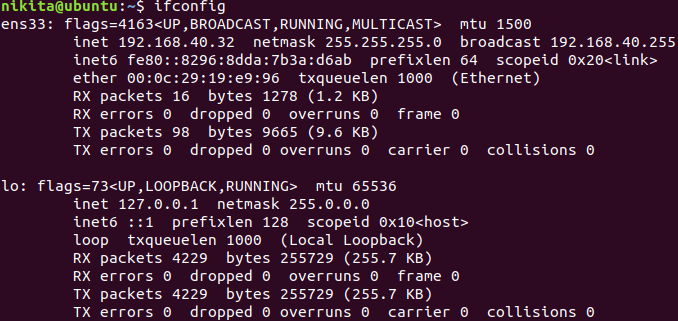
\includegraphics[scale = 0.7]{images/0_1.png}
	\caption{Вывод информации об активных сетевых адаптерах}
	\label{image:0}
\end{figure}

\subsection{Утилита arp}

Утилита командной строки arp используется для отображения и изменения таблиц преобразования IP-адресов в физические (MAC-адреса), используемые протоколом разрешения адресов (Address Resolution Protocol - ARP). 

\begin{figure}[h!]
	\centering
	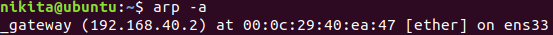
\includegraphics[scale = 0.95]{images/0_2.png}
	\caption{Вывод arp таблицы}
	\label{image:1}
\end{figure}

\subsection{Утилита netstat}

Утилита netstat предназначена для получения оперативной и статистической информации о состоянии сети. Она может выводить таблицу маршрутизации, активные подключения, открытые клиентские и серверные сокеты и др.

\begin{figure}[h!]
	\centering
	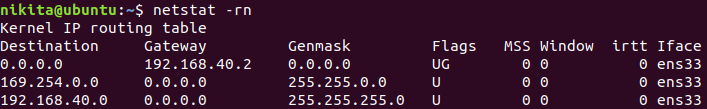
\includegraphics[scale = 0.95]{images/0_3.png}
	\caption{Вывод таблицы маршрутизации}
	\label{image:2}
\end{figure}

\subsection{Утилита hostname}

Утилита hostname устанавливает или отображает символическое имя хоста.

\begin{figure}[h!]
	\centering
	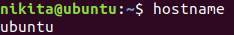
\includegraphics[scale = 0.95]{images/0_4.png}
	\caption{Вывод текущего имени хоста}
	\label{image:3}
\end{figure}

\subsection{Утилита ping}

Утилита ping позволяет определить доступность узла сети при помощи ICMP протокола.

\begin{figure}[h!]
	\centering
	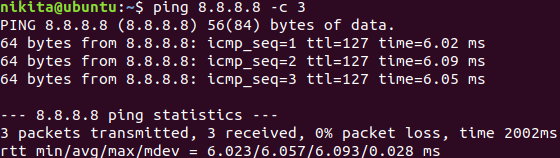
\includegraphics[scale = 0.95]{images/0_5.png}
	\caption{Определение доступности узла 8.8.8.8}
	\label{image:4}
\end{figure}

\clearpage

\subsection{Утилита traceroute}

Утилита traceroute производит трассировку маршрута до конечного узла при помощи наращивания последовательного TTY на ICMP пакетах.

\begin{figure}[h!]
	\centering
	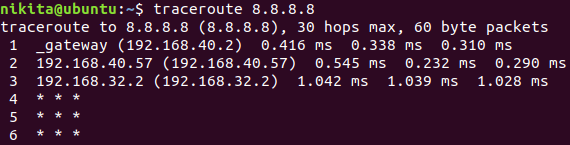
\includegraphics[scale = 0.85]{images/0_6.png}
	\caption{Трассировка маршрута до узла 8.8.8.8}
	\label{image:5}
\end{figure}

\section{Построение карты сети}

Построим карту сети для ККС из предыдущей лабораторной работы. Для этого на Windows XP установим утилиту LanState. При запуске программы, были указаны следующие диапазоны (сегменты сети) для сканирования:

\begin{figure}[h!]
	\centering
	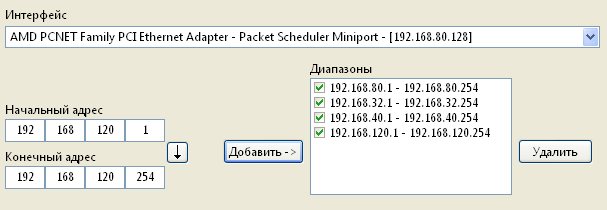
\includegraphics[scale = 0.95]{images/1_1.png}
	\caption{Установка диапазонов сети для сканирования}
	\label{image:6}
\end{figure}

В результате сканирования были найдены следующие узлы:

\begin{figure}[h!]
	\centering
	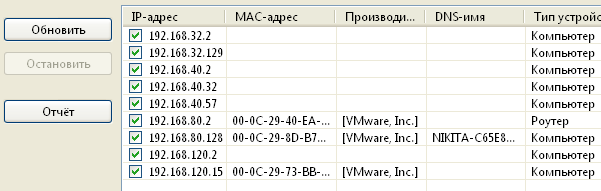
\includegraphics[scale = 0.95]{images/1_2.png}
	\caption{Найденные узлы}
	\label{image:7}
\end{figure}

\clearpage

В результате чего была построена следующая карта сети:

\begin{figure}[h!]
	\centering
	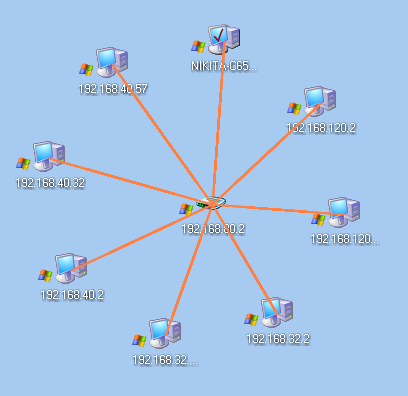
\includegraphics[scale = 0.90]{images/1_3.png}
	\caption{Карта сети}
	\label{image:8}
\end{figure}

Программа не смогла определить точную карту сети, типы операционных систем, она видит лишь ближайший маршрутизатор, в данном случае -- это FreeBSD (хост 192.168.80.2).

\section{Поиск уязвимых узлов}

Для поиска уязвимых узлов на Windows XP установим программу XSpider. При запуске программы, были указаны следующие узлы для сканирования:

\begin{figure}[h!]
	\centering
	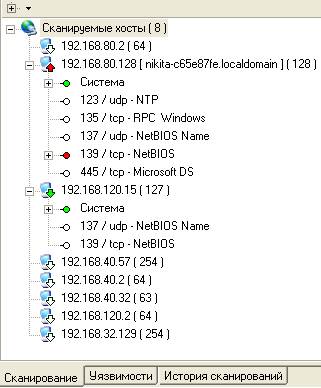
\includegraphics[scale = 0.80]{images/2_1.png}
	\caption{Результат сканирования всех узлов сети}
	\label{image:9}
\end{figure}

Уязвимыми указались узлы с Windows XP и Windows 98. В unix-подобных системах известных уязвимостей не обнаружено.

\section{Оценка пропускной способности}

Оценим пропускную способность через утилиту iperf:

\begin{figure}[h!]
	\centering
	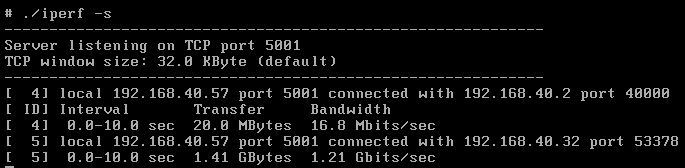
\includegraphics[scale = 0.80]{images/3_0.png}
	\caption{Сервер iperf на NetBSD}
	\label{image:10}
\end{figure}

\begin{figure}[h!]
	\centering
	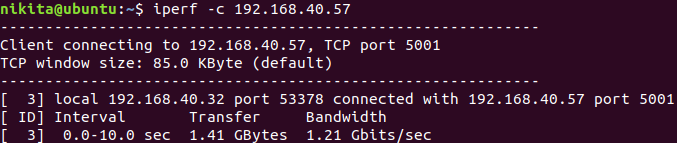
\includegraphics[scale = 0.80]{images/3_1.png}
	\caption{Клиент iperf на Ubuntu}
	\label{image:11}
\end{figure}

\begin{figure}[h!]
	\centering
	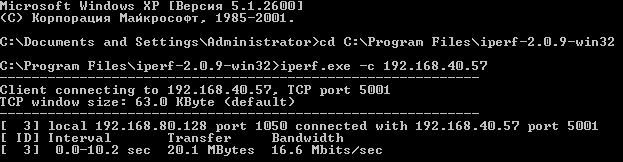
\includegraphics[scale = 0.80]{images/3_2.png}
	\caption{Клиент iperf на Windows XP}
	\label{image:12}
\end{figure}

Пропускная способность узла с Ubuntu оказалась примерно в 75 раз выше, чем у узла с ОС Windows XP.

\section{Вывод}

Построение корректной карты сети оказалось не простой задачей. Помимо шлюза достаточно сложно установить реальную топологию узлов сети.

Поиск уязвимостей наглядно показал, что устаревшие версии операционных систем содержат множество уязвимостей, особенно рассчитанные на пользователя по типу ОС семейства Windows.

Тестирование пропускной способности выявило, что узел с устаревшей Windows XP имеет пропускную способность в 75 раз меньшую, чем узел с обновленной Ubuntu. Такое различие можно попробовать объяснить версией ОС или версией утилиты.

\end{document}